% IEEE standard conference template; to be used with:
%   spconf.sty  - LaTeX style file, and
%   IEEEbib.bst - IEEE bibliography style file.
% --------------------------------------------------------------------------
\documentclass[letterpaper]{article}
\usepackage{amsmath,amssymb,graphicx,spconf}
\usepackage{color}
%\usepackage{listings}


% Example definitions.
% --------------------
% nice symbols for real and complex numbers
%\newcommand{\R}[0]{\mathbb{R}}
%\newcommand{\C}[0]{\mathbb{C}}

% bold paragraph titles
\newcommand{\mypar}[1]{{\bf #1.}}

% Title.
% ------
\title{Belief Propagation for a Recommender System}
%
% Single address.
% ---------------
\name{Elias Sprengel, Frederik Rothenberger, Flurin Rindisbacher, Norman Juchler} 
\address{Department of Computer Science\\ ETH Z\"urich\\Z\"urich, Switzerland}


\begin{document}
%\ninept
\maketitle

\texttt{this should go!}

\begin{abstract}
Belief propagation (BP) is a very general algorithm to perform inference on graphical models. Recently it has been applied in the domain of recommender system by Jiwoon Ha et al.\ (2012). While the results seemed promising, a high computational cost has prevented this method from becoming widely used. In this report we analyse the computational challenges and create a highly optimized version of the BP algorithm that works very well with a recommender system. Our implementation is based on the libDAI library, which provides an excellent code base for BP.
We developed a number of different optimisations which are not only applicable for recommendation engines but can be used to improve the runtime of any application which utilizes BP.
In the end we are able to maintain the high precision of the recommendation system while improving the runtime by a factor of 120, making it feasible to use such recommendation engines in real world applications.
\end{abstract}


\section{Introduction}\label{sec:intro}
%<Introduction of the Introduction>
% NJU:
% I'd emphasise the Belief Propagation, because
% 1) it was the initial motivation to work with this topic
% 2) most of our improvements are applicable to general BP and not just our example

Whether you are planing to segment an image \cite{1544822}, recognize speech \cite{5373446} or analyse medical datasets \cite{bailly2011finding}, belief propagation (BP) plays an important role in all these research areas. This is due to the very general nature of the BP algorithm which allows the user to calculate the probabilities for specific events (a pixel belonging to a region, an audio segment belonging to a language,...). In recent years an other use of BP has been discovered concerning the recommendation of items. Popularized by the Netflix challenge, recommendation systems try to predict which items a user wants to see based on his own ratings and the ratings of other users.

%The work at hand presents a run-time optimized implementation of loopy Belief Propagation, tuned for a Recommender System. In the following, we quickly motivate our work and present the structure of this document.


%Do not start the introduction with the abstract or a slightly modified
%version. It follows a possible structure of the introduction. 
%Note that the structure can be modified, but the
%content should be the same. Introduction and abstract should fill at most the first page, better less.

% Elias: We should keep that in mind because the introduction to the introduction sounds quite similiar to an abstract.

\mypar{Motivation} 
\textit{Belief Propagation} (BP) is a very general and therefore popular algorithm in the domain of machine learning. It has found application in many different areas, ranging from natural to social sciences. 
% Elias: To unspecifc, shouldn't we just include some examples here?
BP is exerted to do probabilistic inference on \textit{graphical models}, out of which Bayesian Networks and Markov Random Fields are the most well known.

The standard version of BP is designed to deal with acyclic graphs. The algorithm can, however, also be applied to graphical models containing loops, although convergence is no longer guaranteed. In this context BP is often called \textit{Loopy Belief Propagation} (LBP). Typical LBP problems are known for bad convergence and high computational costs. Nevertheless the approximated solution is often accurate enough to be used in real world applications.

In this project, LBP is used to build a \textit{Recommender System} (RS). In this system the goal is to generate a list of recommended items for a specific user of a platform or marketplace. The recommendation is based upon the ratings of other users and previous ratings of the user under consideration. With the huge success of online platforms such as Amazon, Youtube and Netflix, Recommender Systems gained a lot of traction in the scientific communities. There exist many different techniques to solve the recommendation problem, some of which build upon BP. [citation] recently proposed such a method. 

A run-time efficient implementation of the RS can be of economic relevance for platforms with large and dynamic user-bases. In the following, we present an analysis on how to achieve this objective for the Top-N Recommender System through loopy BP.

\mypar{Related work} 
As mentioned before, Loopy Belief Propagation methods exhibit bad convergence rates. Worse even, convergence often cannot be guaranteed at all. The illustrative work of Elidan et al. \cite{elidan2012residual} proposes a method to improve both convergence rate and, surprisingly, convergence by itself by propagating belief in an informed way through the graph. The technique is called \textit{Residual Belief Propagation} (RBP) for loopy graphs. RBP is applicable for the Recommender System an therefore is 

We know about two popular open-source C++ frameworks for graph-based inference that implement the message passing algorithm \footnote{This term will be used synonymously for BP in this article.} in a generic way: \textit{libDAI} \cite{Mooij_libDAI_10} on the one hand is a clean and accessible piece of software, whereas \textit{OpenGM} \cite{andres2012opengm} on the other hand is written with a higher degree of abstraction. We chose libDAI as our reference, mostly because it offers a native implementation of RBP (contrary to OpenGM).

In the following, we briefly sketch the Top-N Recommender System based on Residual Belief Propagation in section \ref{sec:background} before we extensively inform the reader in section \ref{sec:method} about the optimization techniques that have applied. The results are presented in section \ref{sec:results}.
\section{Background}\label{sec:background}

%Give a short, self-contained summary of necessary
%background information. For example, assume you present an
%implementation of FFT algorithms. You could organize into DFT
%definition, FFTs considered, and cost analysis. The goal of the
%background section is to make the paper self-contained for an audience
%as large as possible. As in every section
%you start with a very brief overview of the section. Here it could be as follows: In this section 
%we formally define the discrete Fourier transform, introduce the algorithms we use
%and perform a cost analysis.
In this section we introduce the reader to Belief propagation and Top-N Recommendation.

\mypar{Belief Propagation}
Belief Propagation (BP) is a technique in the domain of machine learning to perform probabilistic inference on graphical models, out of which Bayesian Networks and Markov Random Fields are the most well known. The standard version of BP is designed to deal with factor graphs, a bipartite graph that can represent Bayesian Networks or Markov Random Fields. Nodes in a factor graph are either variables or factors. Variable-Nodes hold a belief about the variable assigned to them. A belief is a density function that assigns a probability to each state of the variable/node. Since the number of states of a variable is often finite this belief can be represented as a vector. Factor-Nodes, on the other hand, hold a belief about the joint probabilities of their neighbours. This, for example, means that if there are two Variable-Nodes connected to one Factor-Node the belief of the Factor-Node can be represented as a matrix, where entry $i,j$ holds the belief that one variable is in state $i$ while the other variable is in state $j$. Messages are send to inform neighbouring nodes about the beliefs of the sender. All receivers update their beliefs accordingly and then send updated messages to their neighbours. This is repeated until messages (and therefore beliefs) converge. Conceptually there are two types of messages, from Variable-Nodes to Factor-Nodes and from Factor-Nodes to Variable-Nodes. Understanding the concrete formulas is not required to follow this report but we give both update equations in figure \ref{eqn:bp_message} because they show nicely why this version of the belief propagation is often called the sum product algorithm. As you can see the update equations involve a product over all neighbouring nodes, followed by a sum that marginalizes over all variables excluding the one to which we want to send the message. This sum-product pattern will surface again when we describe our base line implementation in TODO:REF CODE IN SECTION 3.

\begin{figure}
\label{eqn:bp_message}
\begin{equation*}                                                            
\mu_{v\rightarrow a}(x_v) = \prod_{\hat a \in N(v)\backslash \{a\}} \mu_{\hat a\rightarrow v}(x_v)
\end{equation*}
\begin{equation*}                                                            
\mu_{a\rightarrow v}(x_v) = \sum_{x_a \sim x_v}f_a(x_a) \prod_{\hat v \in N(a)\backslash \{v\}} \mu_{\hat v\rightarrow a}(x_{\hat v})
\end{equation*}
\caption{Update equations for the BP algorithm. First for messages from variable node $v$ to factor $a$ and the second for messages from factor $a$ to variable node $v$; $x_v$ is the specific state for which we want to send our belief; $f_a(x_a)$ denotes the belief of the factor node $a$ about state $x_a$; $\mu$ is the message itself; $k \in N(i)\backslash j$ denotes all neighbours of $i$ except the neighbouring node $j$ and $x_a \sim x_v$ is used to denote all possible states that are consistent with state $x_v$.}
\end{figure}

The standard version of BP is designed to deal with acyclic graphs. The algorithm can, however, also be applied to graphical models containing loops, although convergence can no longer be guaranteed. In this context BP is often called \textit{Loopy Belief Propagation} (LBP). LBP problems are known for bad convergence and high computational costs. Nevertheless the approximated solution is often accurate enough to be used in real world applications. The illustrative work of Elidan et al. \cite{elidan2012residual} proposes a method to improve both convergence rate and, surprisingly, convergence (Elias TODO: convergence, not accuracy? Don't get it) by itself by propagating belief in an informed way through the graph. The technique is called \textit{Residual Belief Propagation} (RBP) for loopy graphs because a residual for each message is computed.
(Elias TODO: How is the residual computed? I want to write something like it reflects the importance of updating the message and we, therefore, should always update the message with the highest residual, but I'm not sure that is correct.)


\mypar{Top-N Recommendation}
Top-N Recommendation is the problem of generating a list of recommended items for a user $\hat u$. The list is based on the ratings of the user $\hat u$ as well as the ratings of the other users. Ha et al. \cite{Ha:2012:TRT:2396761.2398636} propose a method for Top-N Recommendation using loopy belief propagation. In this method the factor graph contains variable nodes for every users and every movies. The state of each node can either be\\
'1: $\hat u$ likes this user/movie' or\\
'2: $\hat u$ does not like this user/movie'. \\
Factors are used to connect movies with users. In more detail: we take all the ratings that are above average, meaning that a user $u_i$ really liked a movie $m_j$. We then create a factor connecting $u_i$ with $m_j$. This factor will have four states (2x2 matrix). We set the values $(1,1)$ and $(2,2)$ to $0.5 + \alpha$, $alpha = 0.0001$ to denote our belief that if user $\hat u$ likes either the movie $m_j$ or the user $u_i$, he will probably like the other one as well (transitivity of 'like'). Furthermore we set $(1,2)$ and $(2,1)$ to $0.5 - \alpha$ to express our belief that it is unlikely that user $\hat u$ only likes the movie or the user but not both.
Furthermore we already know a few movies that $\hat u$ likes/dislikes. This means for every rating from $\hat u$ for movie $m_j$ we set the belief of node $m_j$ to reflect that rating. In our concrete example ratings could vary between 1 and 5 stars which meant we would map a rating of 5 to $[0.9,0.1]$, a rating of 4 to $[0.7,0.3]$, 3 to $[0.5,0.5]$, 2 to $[0.3,0.7]$ and 1 to $[0.1,0.9]$. All other beliefs are initialized with $[0.5,0.5]$.

Figure \ref{top_n_graph} shows a small factor graph for  $\hat u = u_2$ where user $u_1$ has rated the movies $m1,m2$, $u_2$ the movie $m_2$ and $u_3$ the movies $m_1,m_2$ and $m_3$. Initially it is only known, that user $u_2$ likes the movie $m_2$ with a probability of 0.7. 
Using loopy belief propagation the most important messages are sent through the factors and the belief is propagated from observed nodes to unobserved nodes (see Figure \ref{top_n_graph_important_msg}). When the belief propagation converges each movie has a probability "User $\hat u$ likes movie $j$". Figure \ref{top_n_graph_final_state} shows a possible final state. The movies can be sorted by these probabilities and the top N elements are returned. In this example movie $m_1$ would be the top-one recommendation for user $u_2$.

% TODO why u no horizontal display?
\begin{figure}[h]\centering

%\subfloat{
    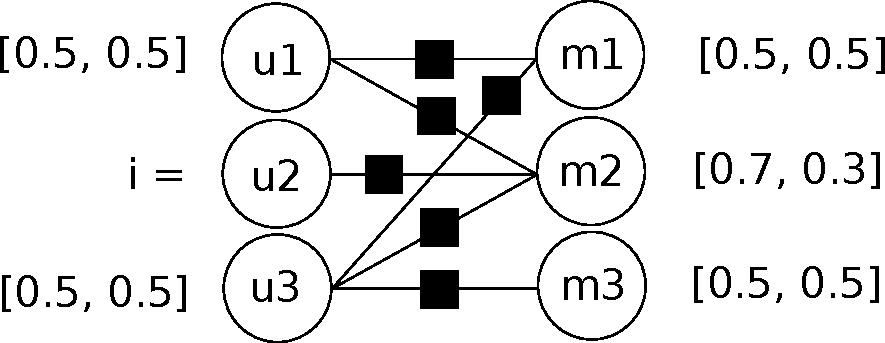
\includegraphics[scale=0.33]{graphics/top-n-graph.pdf}
\caption{Factor Graph for predicting top-n movies for user $u_2$. The dark squares are the factors. The values in [] show the probabilities for the random variables being in state "like" or "don't like".\label{top_n_graph}}
 %}

%\subfloat{
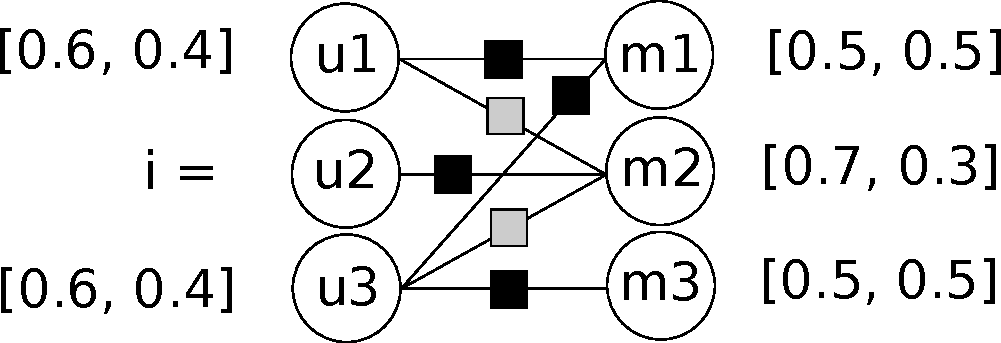
\includegraphics[scale=0.33]{graphics/top-n-important-messages.pdf}
  \caption{Belief is propagated from observed node $m_2$ to unobserved notes \label{top_n_graph_important_msg}}
  %} 

    %\subfloat{
    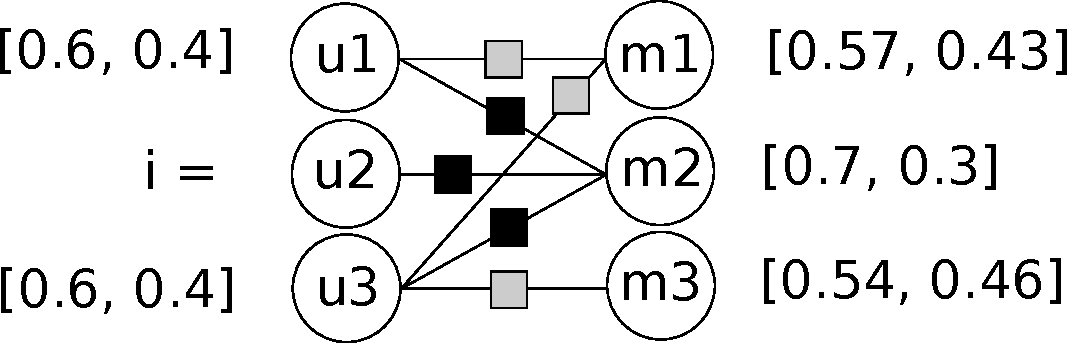
\includegraphics[scale=0.33]{graphics/top-n-final.pdf}
  \caption{A possible final state for top-n recommendation. Movie $m_1$ is the top recommendation for user $u_2$. \label{top_n_graph_final_state}}
%  }

\end{figure}

\mypar{Cost Analysis}

\textbf{TODO}

%\mypar{Discrete Fourier Transform}
%Precisely define the transform so I understand it even if I have never
%seen it before.
%
%\mypar{Fast Fourier Transforms}
%Explain the algorithm you use.
%
%\mypar{Cost Analysis}
%First define you cost measure (what you count) and then compute the
%cost. Ideally precisely, at least asymptotically. In the latter case you will need to instrument your code to count
%the operations so you can create a performance plot.
%
%Also state what is
%known about the complexity (asymptotic usually) 
%about your problem (including citations).
\section{Proposed Method}\label{sec:method}

%Now comes the ``beef'' of the paper, where you explain what you
%did. Again, organize it in paragraphs with titles. As in every section
%you start with a very brief overview of the section.

%For this class, explain all the optimizations you performed. This mean, you first very briefly
%explain the baseline implementation, then go through locality and other optimizations, and finally SSE (every project will be slightly different of course). Show or mention relevant analysis or assumptions. A few examples: 1) Profiling may lead you to optimize one part first; 2) bandwidth plus data transfer analysis may show that it is memory bound; 3) it may be too hard to implement the algorithm in full generality: make assumptions and state them (e.g., we assume $n$ is divisible by 4; or, we consider only one type of input image); 4) explain how certain data accesses have poor locality. Generally, any type of analysis adds value to your work.
As a baseline we used the libDai library \cite{Mooij_libDAI_10} which provides an implementation for loopy belief propagation using the max residual updating scheme. Using the library is was easy to implement a recommendation system on top of it, closely following \cite{Ha:2012:TRT:2396761.2398636}. One important decision, when dealing with belief propagation, is the one concerning the domain. Switching to a logarithmic domain enables us to express the product over the messages as a sum, often making it less likely to suffer from numerical rounding errors and sometimes making the computation faster. We tested both methods and decided to not utilize the logarithmic domain because the accuracy did not increase and the overhead of transforming the results from/to the log-domain gave us a small increase in the runtime. 

\mypar{Code structure}
Figure \ref{overviewflow} shows a very high level overview of our code structure. After an initialization phase the belief propagation algorithm is invoked. The algorithms then loops until a specified number of maximum iteration is reached, the maximum residual becomes zero or the change in the updated messages is smaller than some specified tolerance. In every iteration 'findMaxResidual' is called to determine the message which should be updated next. After the message is determined it gets updated with a call to 'updateMessage' which also calls 'updateResidual' to update the corresponding residual. This can be done quickly because we already store not only the current messages for each node but also the new message in a container called 'newMessages'. Therefore 'updateMessage' only needs to set the current message to the new one. Finally all messages inside the 'newMessages' container that would be affected by this change needs to be recomputed. We call 'calcNewMessage' which goes through the neighbourhood of the updated message and recomputes the messages, storing the updated version in our 'newMessages' container. In order to compute the new message we first need to compute a product over all incoming messages which is done in 'calcIncomingMessageProduct'. Because we are only interested in a single variable the product is then marginalized (over all other variables) which is done with a call to 'marginalizeProductOntoMessage'. We observe that the methods that get called the most often are 'updateResidual', 'calcIncomingMessageProduct' and 'marginalizeProductOntoMessage'. This is why our optimizations will mostly focus on these.

\begin{figure}\centering
    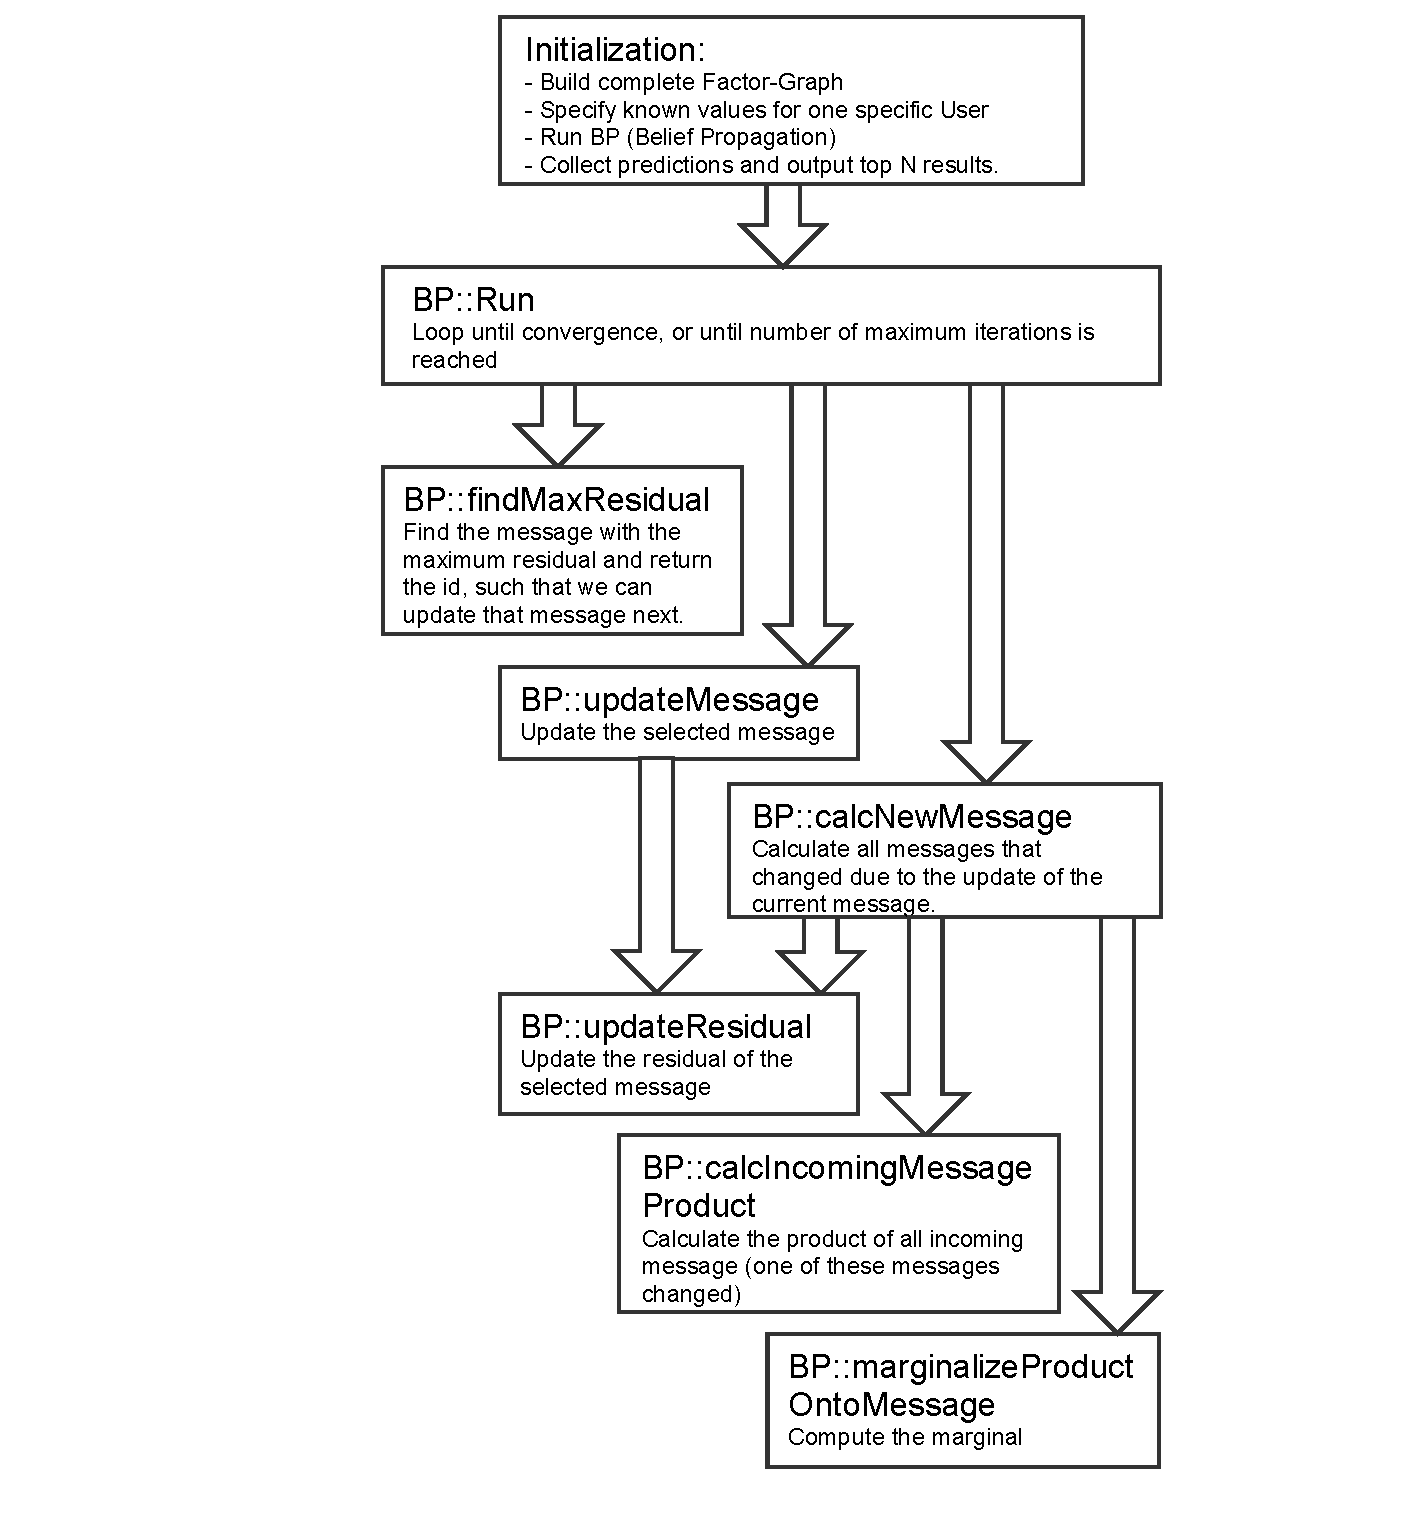
\includegraphics[scale=0.63, trim={6.5cm 0cm 0 0cm},clip]{graphics/loopybp.pdf}
  \caption{Flow (top to bottom) of our program. Arrows denote that a methods gets called from an other, BP is the namespace used for all functions that deal with belief propagation.\label{overviewflow}}
\end{figure}


\mypar{Optimizations}

After we created our baseline and set up a testing environment to automatically validate all our changes we started with the optimizations. We tried to focus on general optimizations first that wouldn't change the interface/functionality of the library. After that was done we focused on our concrete example (recommendation), trading in generality for speed, drastically changing the interface and functionality of the library. In both parts we started with optimizations concerning the number of flops, without considering the computational intensity. We then profiled our code to find critical points where we could optimize memory access patterns or reorder operations to increase the computational intensity. This was also the point where we decided to switch from double to single precision which decreased our accuracy slightly but gave us an significant boost for the runtime. %TODO: How much?
As a final step we considered vectorization which gave us only a very small speed-up. We will know explain all our optimizations in more detail.
 
\mypar{General optimizations}
We started with optimizations that could be applied without changing or limiting the functionality of the library.

The first issue was that we are recomputing the incoming message product every time a message gets updated. This is wasteful because the product could include well over a hundred factors from which only one would change. To avoid the re-computation we compute the product once over all messages. Whenever a message changes we also update the product by multiplying it with the new message and dividing it by the old message. This gave us an speed-up of 1.6 reducing the runtime of the algorithm from 80 to 50 seconds.

Next Norman did a bunch of stuff...

\mypar{Specific optimisations}
Floats -> Double = specific because it changes the result, not okay for a library

Pattern 0101 and 0011

Used the fact that we only stored p, 1-p

Residual

Vectorization
%As important as the final results is to show that you took a structured, organized approach to the optimization and that you explain why you did what you did.

%Mention and cite any external resources including library or other code.

%Good visuals or even brief code snippets to illustrate what you did are good. Pasting large amounts of code to fill the space is not good.

\section{Experimental Results}\label{sec:results}

\mypar{Experimental setup} The improvements were evaluated on two different platforms:
\begin{itemize}
\item Intel\textsuperscript{\textregistered} Xeon CPU E3-1220L V2 @ 2.30 GHz, gcc (Debian 4.9.2-10) 4.9.2
\item Intel\textsuperscript{\textregistered} Core i5-2500 @ 3.3 GHz, Windows 8.1 using cygwin64 with gcc 4.9.2
\end{itemize}

The program versions were compiled with the following flags: 
-std=c++11 -Wno-deprecated -Wall -W -Wextra -fPIC -march=native -O3 -DNDEBUG -fPIC
\\
For performance analysis Intel\textsuperscript{\textregistered} VTune Amplifier XE 2015 (build 403110) was used. Cycle counts were compared with the readings obtained by using the RDTSC instruction to check the accuracy of VTune Amplifier XE 2015. Measurements deviated by less than 1\%.

\mypar{Baseline}
The analysis of the baseline implementation showed a lot of potential for optimization. Most notably by reducing memory overhead caused by object creation and deletion, random reads from lookup tables and vector operations. This can also be seen in the roofline analysis \cite{Ofenbeck:14} (see figure~\ref{roofline-mixed}).

\mypar{Impact of Optimizations}
As can be seen in figure~\ref{runtime}, the overall runtime was reduced by a factor of 8.7 to 27.4 depending on input size. Most of these improvements were achieved by reducing the number of operations by a factor of 13.5 as shown in figure~\ref{flops-per-message}. One particular optimization (build 6 in figure~\ref{runtime}) replaced many multiplications with one division. Due to such optimizations the performance of the optimized version did not improve, as indicated by the roofline analysis in figure~\ref{roofline-mixed}. Furthermore by reducing the op count and introducing divisions the division unit became a bottle neck.

\mypar{Memory Accesses}
Despite all the optimizations some operations (e.g. retrieving the greatest residual to determine which message to process next or graph lookup operations) are inherently non linear in memory. These operations are expensive as they access random memory locations. This is especially an issue if the factor graph is larger than 1 MB as then the TLB (in the systems we measured with) can no longer serve all address translations for the graph accesses.

\begin{figure}\centering
    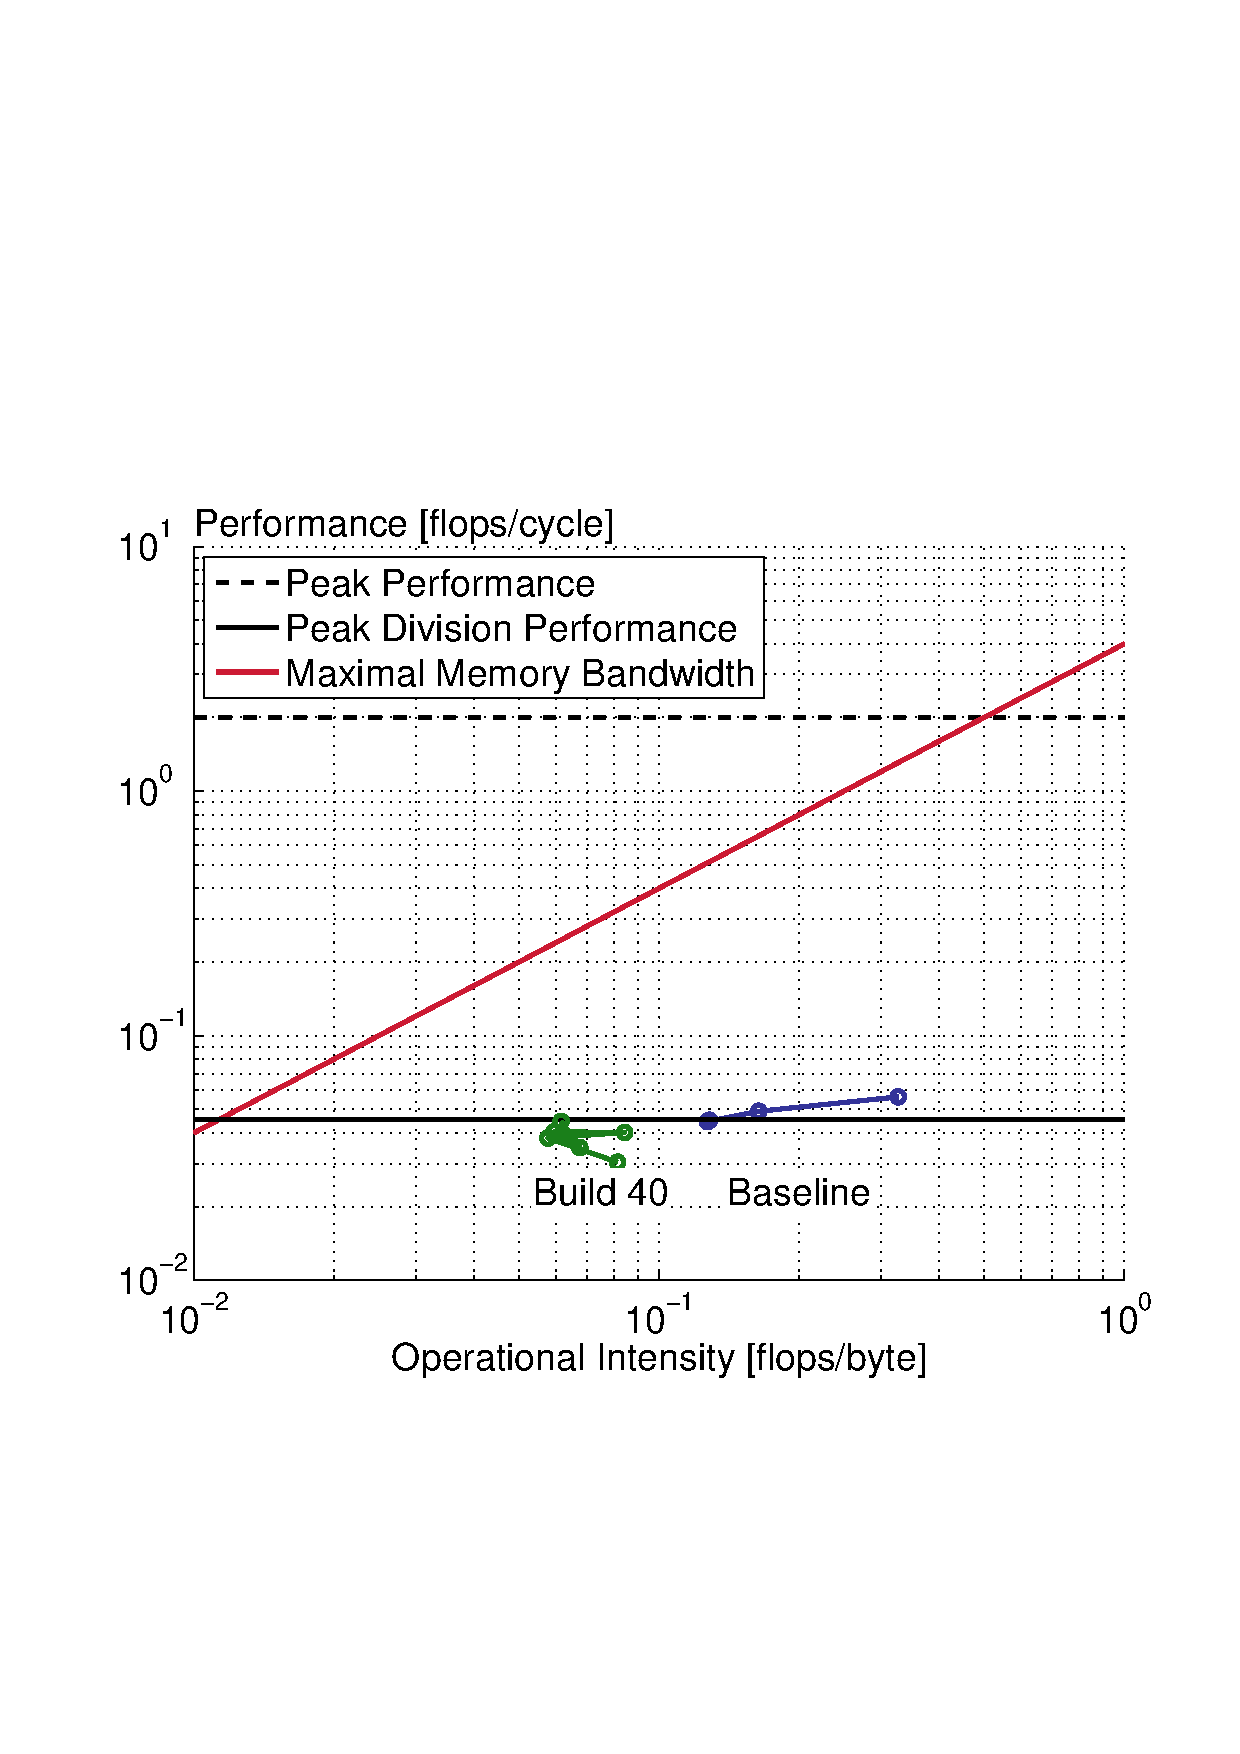
\includegraphics[scale=0.47, trim={1.9cm 6cm 1.1cm 8.5cm},clip]{graphics/roofline_mixed.pdf}
  \caption{Roofline analysis of the baseline and our optimized version (build 40). The analysis was conducted on the Windows system described above.\label{roofline-mixed}}
\end{figure}

\begin{figure}\centering
    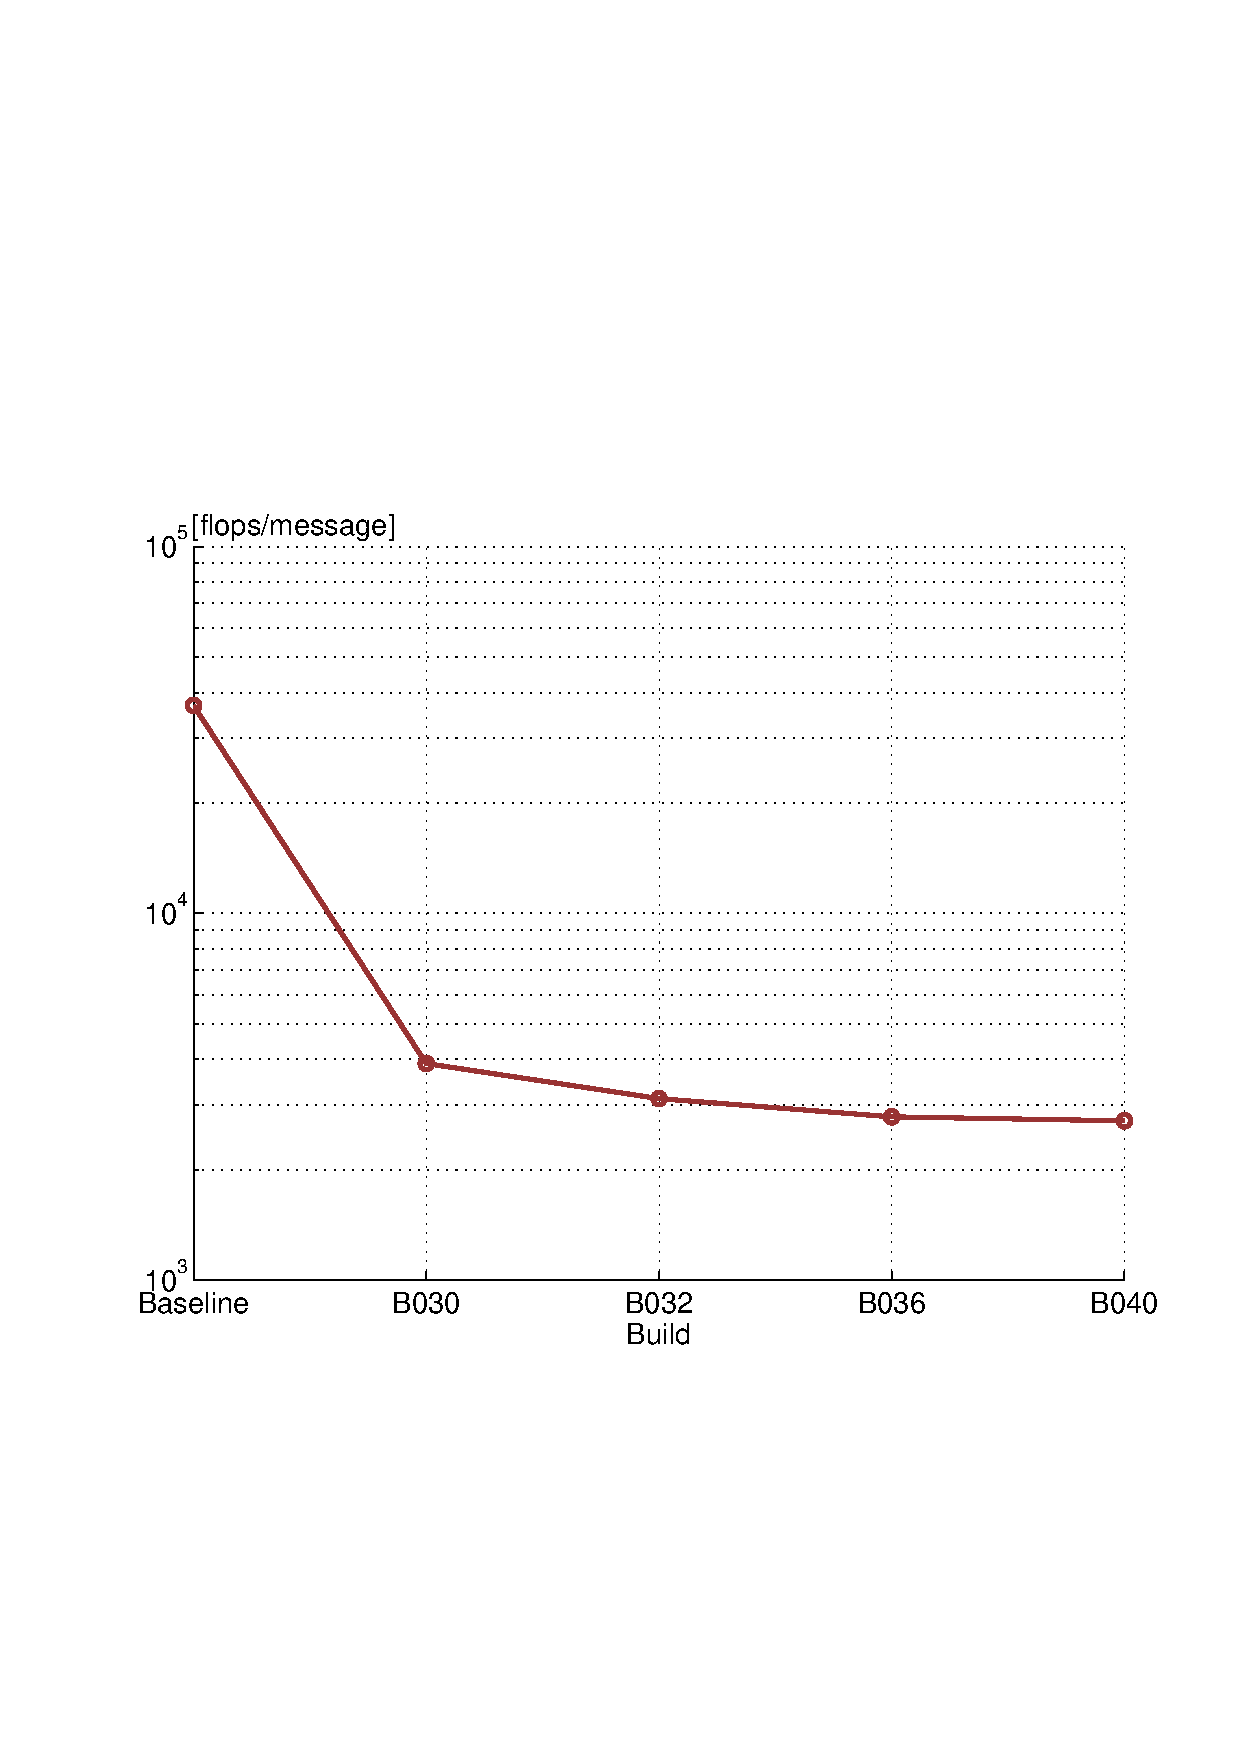
\includegraphics[scale=0.47, trim={1.9cm 6.5cm 1.1cm 8.5cm},clip]{graphics/flops_per_message.pdf}
  \caption{Comparison of the number of floating point operations needed to update a single message for different builds of the program.\label{flops-per-message}}
\end{figure}

\begin{figure*}\centering
  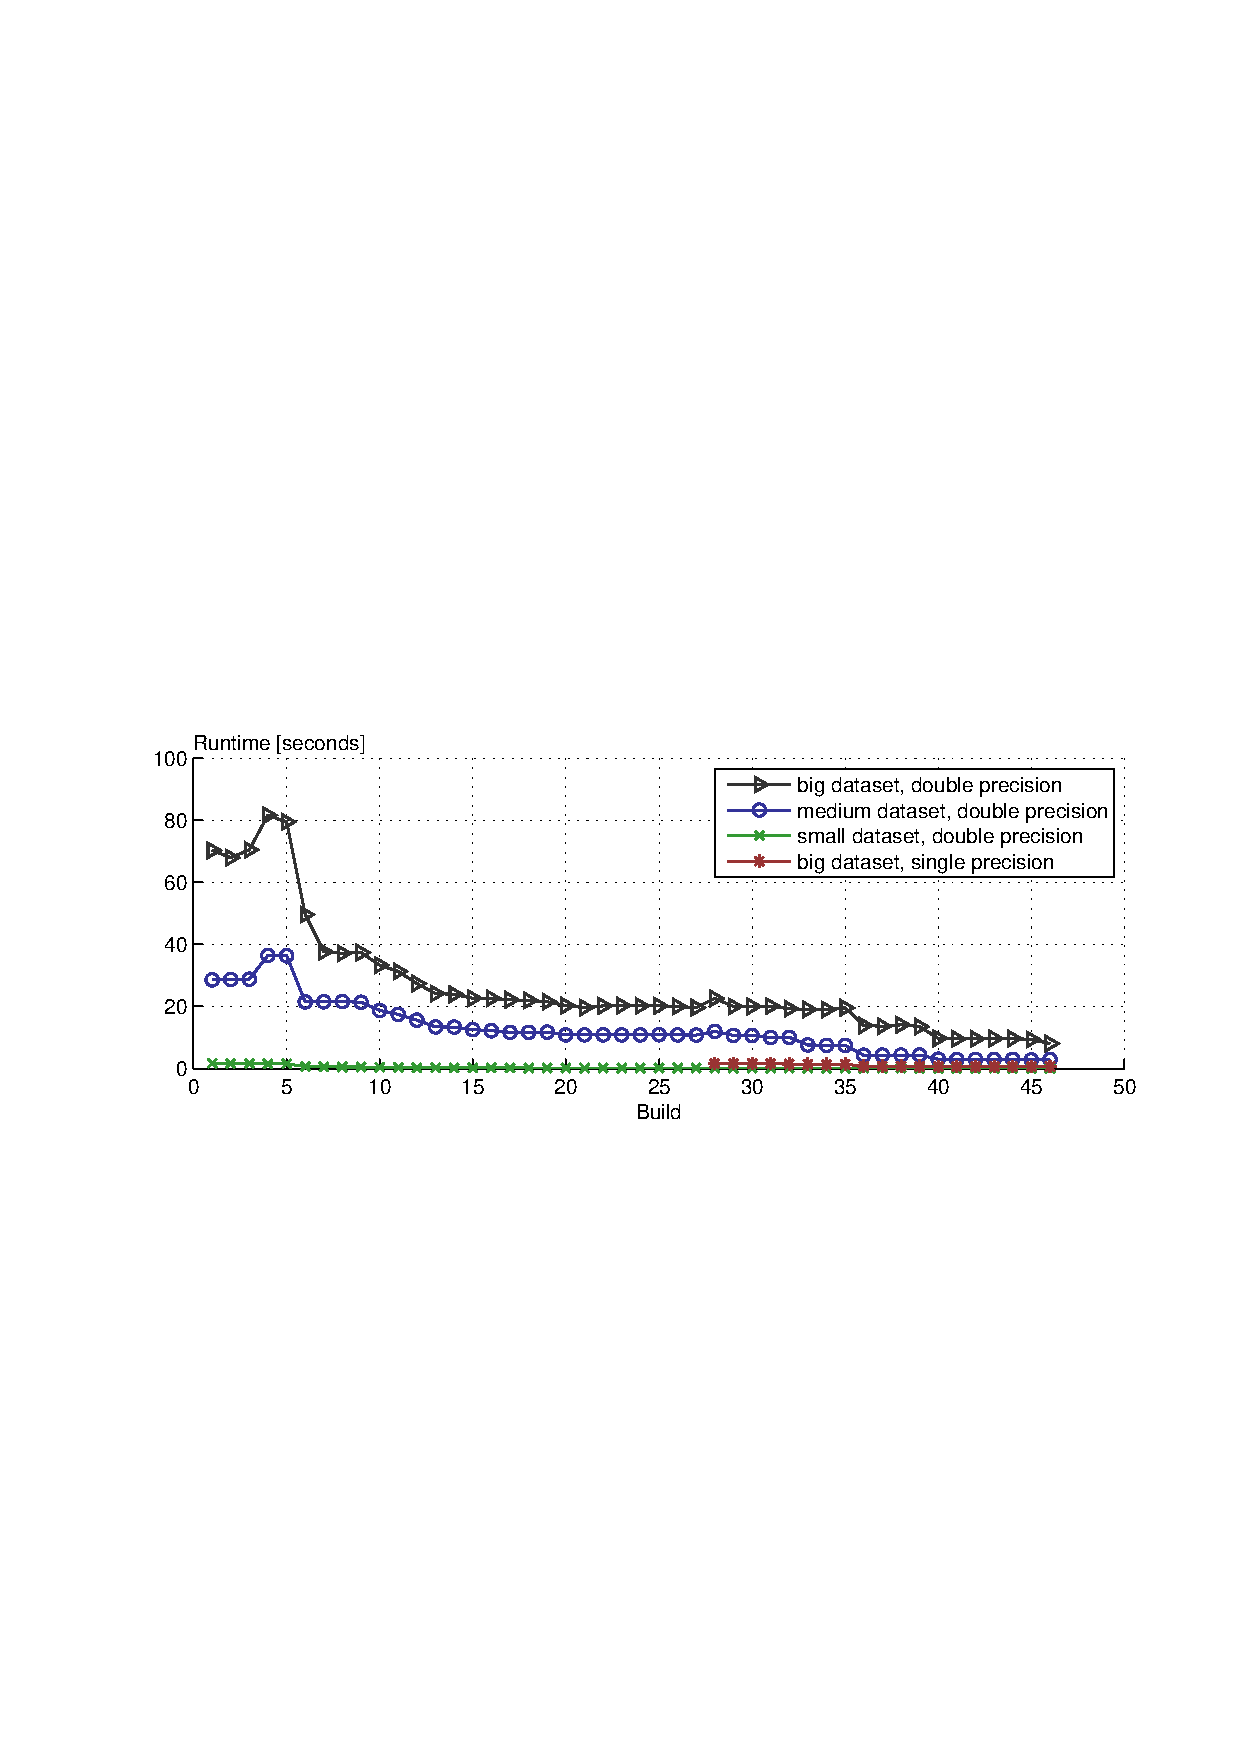
\includegraphics[scale = 1, trim={7cm 11cm 6.4cm 14cm}]{graphics/runtime_plot.pdf}
  \caption{Runtime plot showing the execution time on the Linux system across different versions of our program for three different input sizes. Dataset details: big: 80367 ratings, 943 users, 1683 movies; medium: 33392 ratings, 943 users, 272 movies; small: 3594 ratings, 943 users, 32 movies.\label{runtime}}
\end{figure*}

\mypar{Vectorization}
To further improve the runtime some parts of the code were vectorized manually. Unfortunately, this did not bring a significant improvement, due to some difficulties:
\begin{itemize}
	\item The op count was reduced significantly by replacing floating point multiplications with floating point divisions (by reusing previously calculated products). This lead to a performance bound by the division unit.
	\item Vectorizing this division is not possible as the program flow depends on the result immediately, thus calculation 4 divisions at once is impossible. This dependency stems from the fact that the residuals are influenced by the result of the division. And calculating only one division using AVX is slower than a scalar division \cite{intrinsics_guide}.
	\item Doing a scalar division results in a dependency on the write back of the floating point vector, which is expensive.
\end{itemize}

\section{Conclusions}
We showed that pre computing values, optimizing memory accesses, loop unrolling together with scalar replacements and vectorization lead to speed-up by a factor of 8.7 to 27.4 depending on input. For our Top-N recommendation system this means that we improved the runtime on on our big dataset from 21 hours to about 45 minutes. Even better, by switching to single precision we are able to maintain the same accuracy on the predictions while reducing the runtime by yet an other factor of 6, down to about 8 minutes. We believe that this shows that the idea of applying belief propagation to recommender system is not only theoretical in nature but can be applied in real world systems. Furthermore a lot of our optimisations apply not only to our concrete example but are more general. Our empirical results show that implementing those improves the BP runtime of the library by a factor of 3. Because the libDai library is widely used for belief propagation a lot of applications can benefit from our optimisations. Especially because in most applications BP takes up a significant portion of the runtime.

\section{Further comments}

Here we provide some further tips.

\mypar{Further general guidelines}

\begin{itemize}
\item For short papers, to save space, I use paragraph titles instead of
subsections, as shown in the introduction.

\item It is generally a good idea to break sections into such smaller
units for readability and since it helps you to (visually) structure the story.

\item The above section titles should be adapted to more precisely
reflect what you do.

\item Each section should be started with a very
short summary of what the reader can expect in this section. Nothing
more awkward as when the story starts and one does not know what the
direction is or the goal.

\item Make sure you define every acronym you use, no matter how
convinced you are the reader knows it.

\item Always spell-check before you submit (to me in this case).

\item Be picky. When writing a paper you should always strive for very
high quality. Many people may read it and the quality makes a big difference.
In this class, the quality is part of the grade.

\item Books helping you to write better: \cite{Higham:98} and \cite{Strunk:00}.

\item Conversion to pdf (latex users only): 

dvips -o conference.ps -t letter -Ppdf -G0 conference.dvi

and then

ps2pdf conference.ps
\end{itemize}

\mypar{Graphics} For plots that are not images {\em never} generate (even as intermediate step)
jpeg, gif, bmp, tif. Use eps, which means encapsulate postscript, os pdf. This way it is
scalable since it is a vector graphic description of your graph. E.g.,
from Matlab, you can export to eps or pdf.

Here is an example of how to get a plot into latex
(Fig.~\ref{fftperf}). Note that the text should not be any smaller than shown.

\begin{figure}\centering
    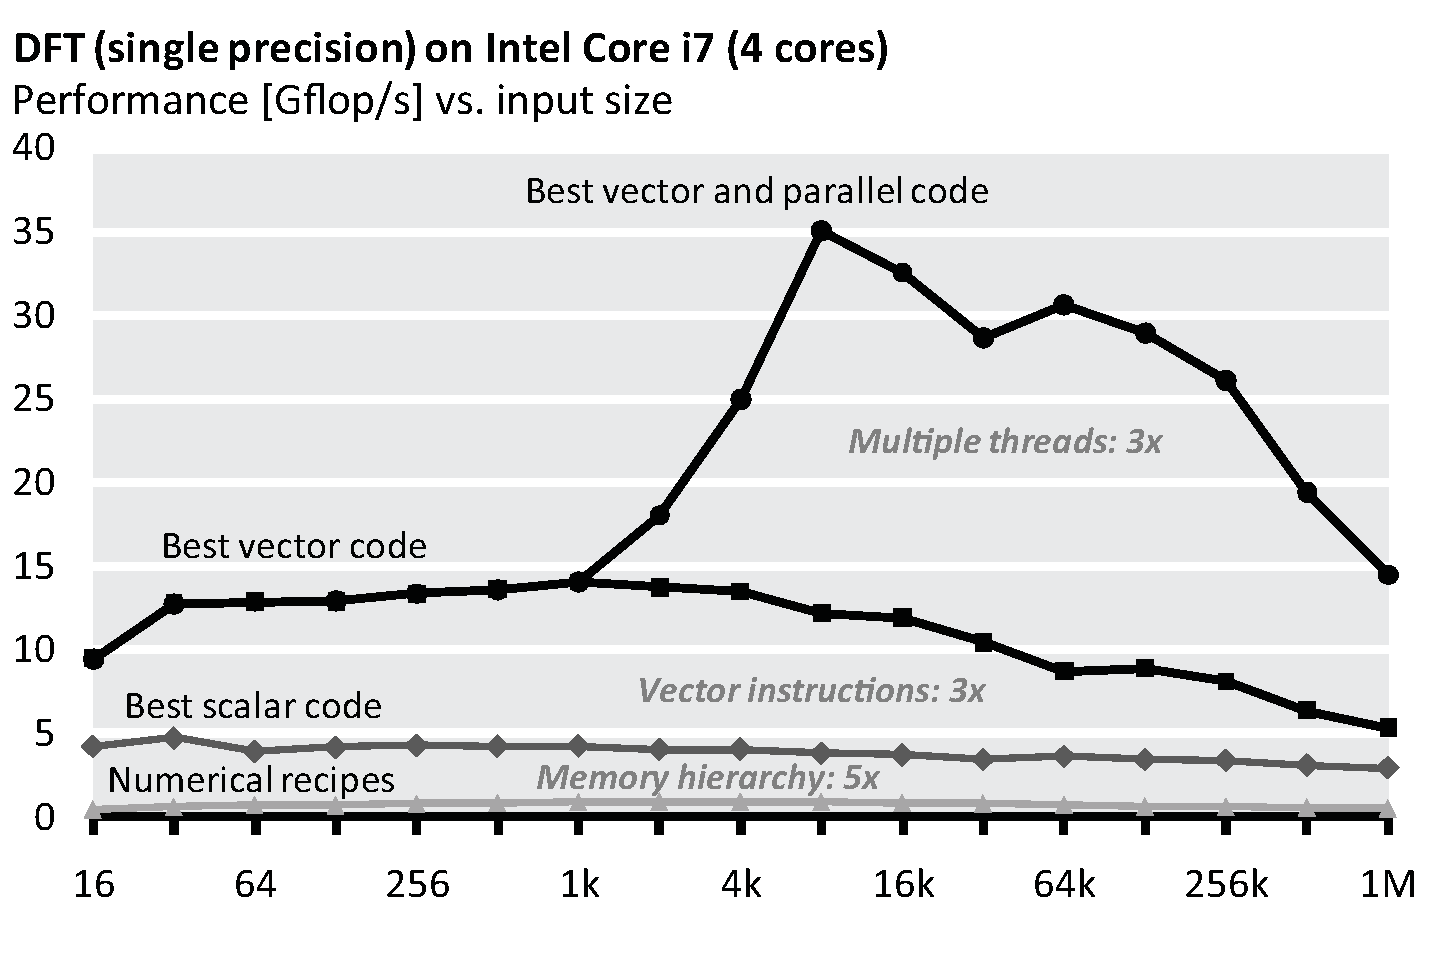
\includegraphics[scale=0.33]{graphics/dft-performance.pdf}
  \caption{Performance of four single precision implementations of the
  discrete Fourier transform. The operations count is roughly the
  same. {\em The labels in this plot are too small.}\label{fftperf}}
\end{figure}




% References should be produced using the bibtex program from suitable
% BiBTeX files (here: bibl_conf). The IEEEbib.bst bibliography
% style file from IEEE produces unsorted bibliography list.
% -------------------------------------------------------------------------
\bibliographystyle{IEEEbib}
\bibliography{bibl_conf}

\end{document}

